
\section*{Resources \& Networking}
\DefineNamedColor{named}{eclipsered}{rgb}{0.386,0.366,0.682}
\definecolor{tablecolor}{named}{eclipsered}


\subsection*{Getting Gear}

\begin{eptable}{ X }
   \epheader{1}{Before Missions}
   Regular mission has 20 GP and 6 MP, but adjust accordingly.\\
   GP can only be spent in mission prep phase, can't be saved.\\
   Resource trait level adds to GP.\\
   Favors can be traded for 1 to 3 GP, if rep 40+ and appropriate.\\
\end{eptable}

\bigskip

\begin{eptable}{ X }
   \epheader{1}{During Missions}
   Spend regular rep favors for gear (minor to major).\\
   Use resource trait to buy.\\
   Find and use nanofabricator to build if blueprints available.\\
\end{eptable}

\bigskip

\begin{eptable}{ l | X }
   \epheader{2}{Resource Trait During Missions}
   Level 1 & Up to 2 GP per week on minor items.\\
   Level 2 & Up to 3 GP per week on minor or moderate items.\\
   Level 3 & Up to 5 GP per week on any complexity.\\
   Level 4 & Same as Level 3, but also rare or restricted (pending GM).\\
\end{eptable}

\bigskip

\begin{figure}[htb!]%
   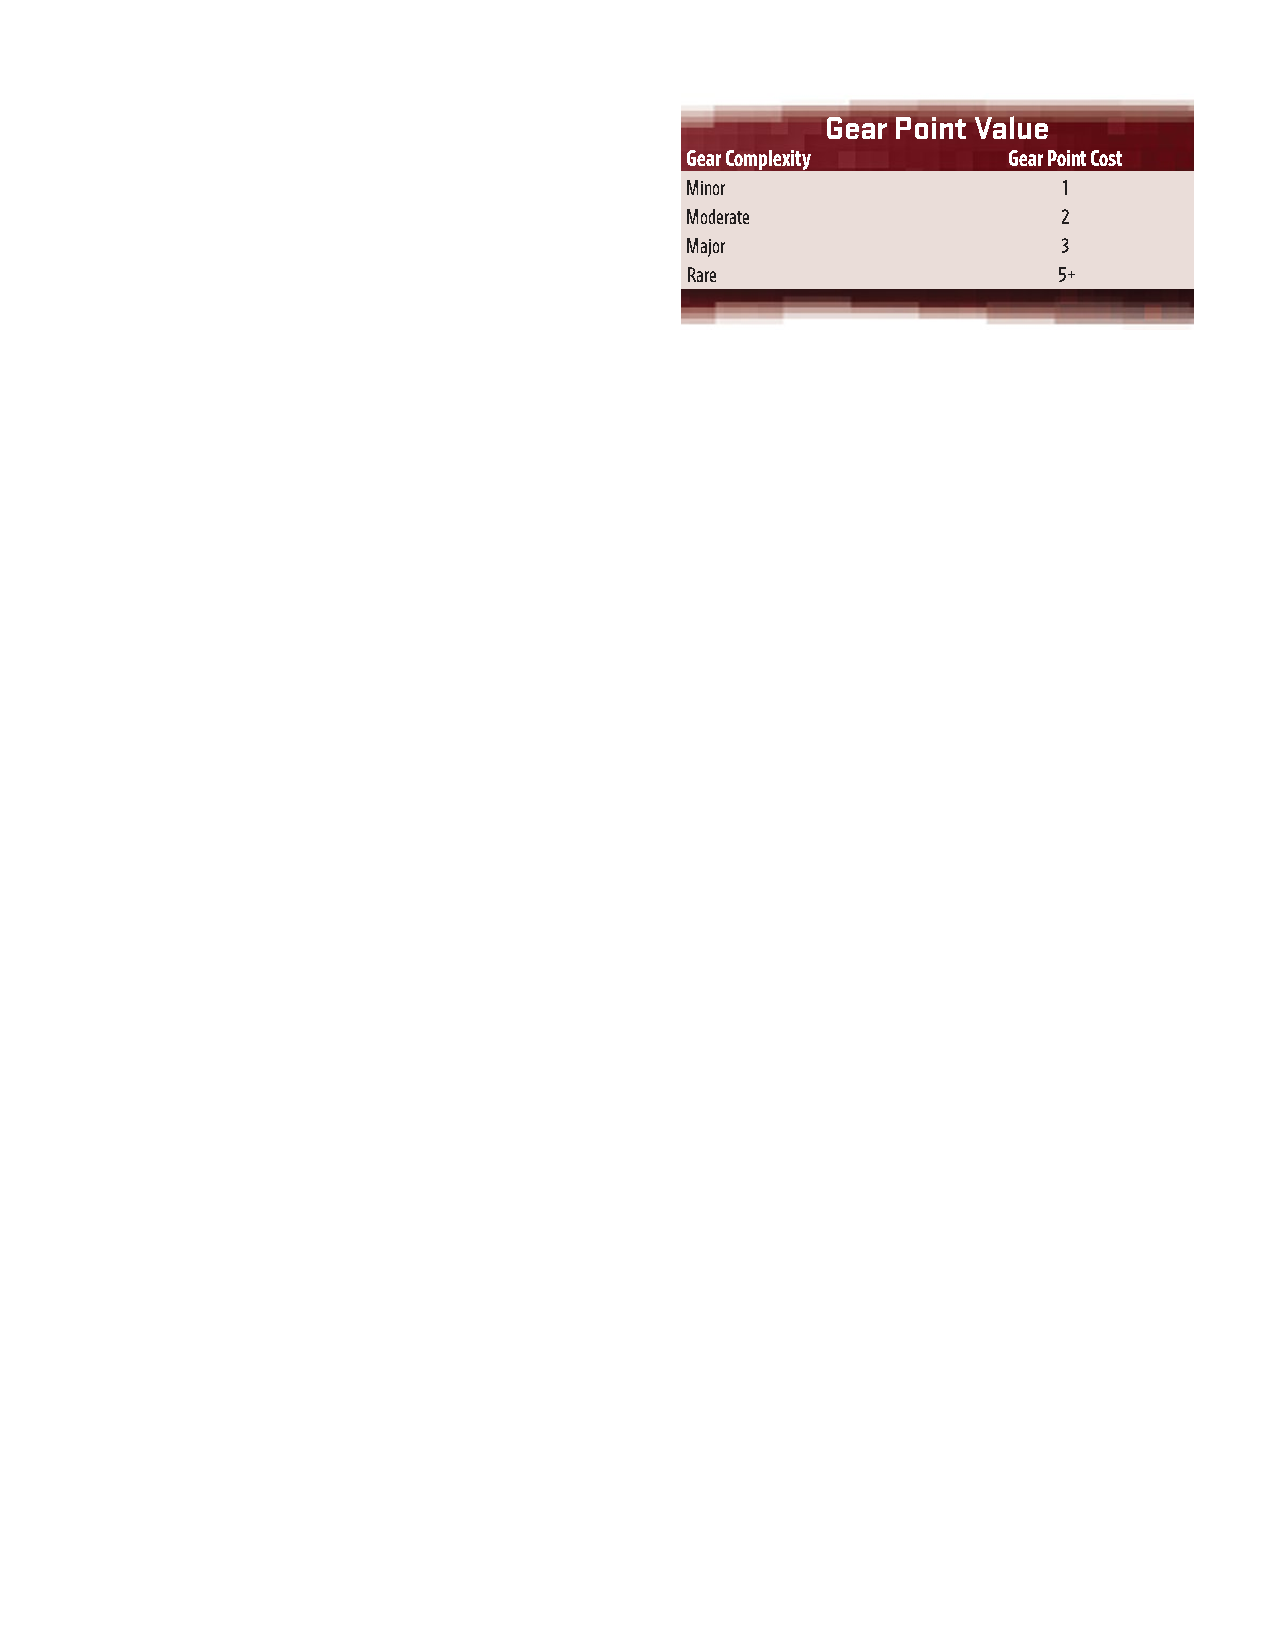
\includegraphics[scale=0.95]{gfx/resources-rep-gearpoints}%
\end{figure}%

\begin{itemize}
    \itembox \textbf{Time.} In general cases it is just a matter of
    waiting. In special cases a \skill{Persuation} test may be needed. Acquiring multiple items combines time frame.
    \itembox \textbf{Blueprints.} When acquiring gear, chose between actual item or single-use blueprint. Multi-use blueprints are available, but increase complexity by one step. Regular blueprints are assumed to come with one physical copy.
    \itembox \textbf{Flex.} At Level 3 and Level 4 can be used with Flex to immediately
            acquire Moderate items and introduce them to the scene.
    \itembox \textbf{Bribing.} High traits can also be used as bribing modifier in
        certain situations. Apply \modifier{+10} per level of trait.
\end{itemize}

\bigskip


\begin{eptable}{ l | X }
   \epheader{2}{Resource Trait \& Life Style}
   Level 1 & Own cubicle in a beehive hab or a small apartment.\\
   Level 2 & Private residence or a condo. Small vehicle.\\
   Level 3 & Large residential complex or multiple homes, one or more vehicles.\\
   Level 4 & Rich, might own a small private hab and even shuttle.\\
\end{eptable}


\bigskip

\begin{figure}[htb!]%
   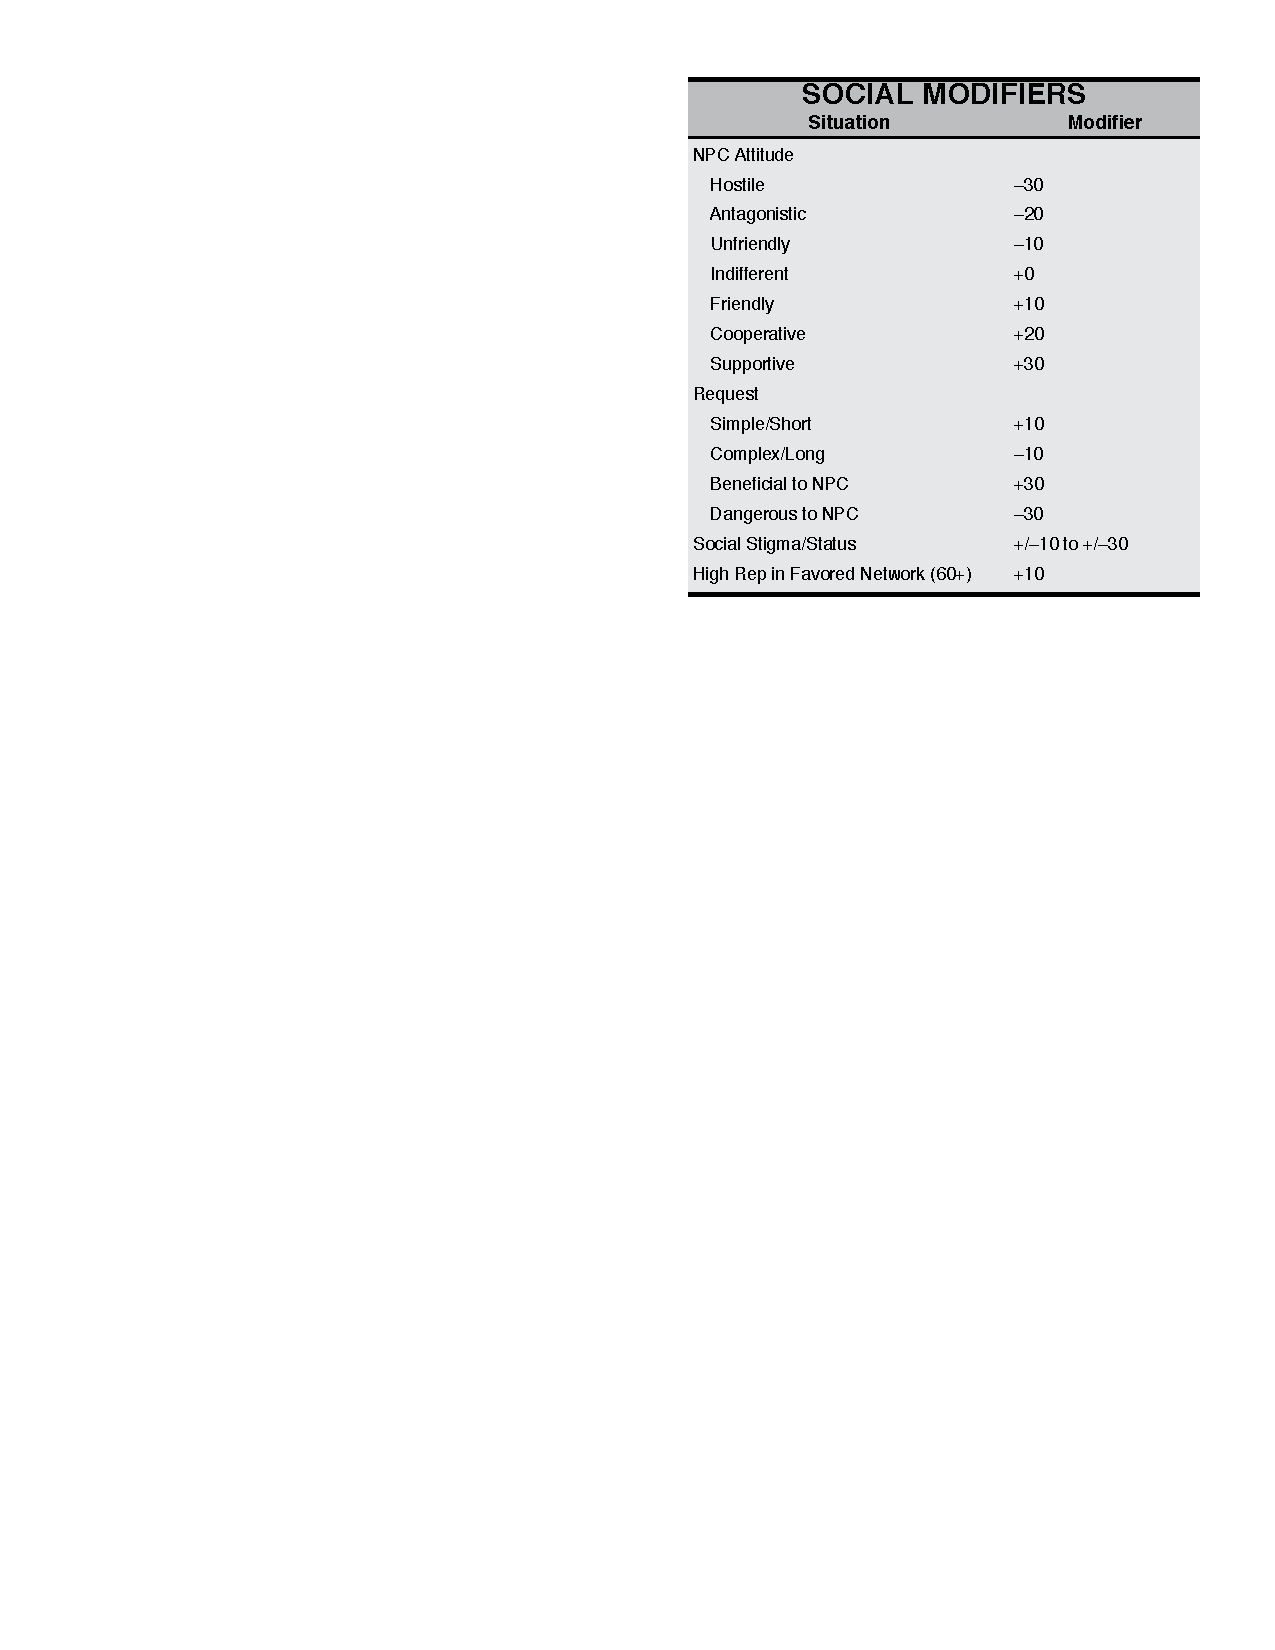
\includegraphics[scale=0.95]{gfx/combat-social-modifiers}%
\end{figure}%




\begin{eptable}{ l | X }
   \epheader{2}{Acquisition Time Frame}
   Digital Only & \num{1} minute.\\
   Minor & \num{2} hours.\\
   Moderate & \num{8} hours.\\
   Major & \num{24} hours.\\
   Rare, Restricted & GM choice.\\
\end{eptable}

\bigskip


\begin{eptable}{ l | X }
   \epheader{2}{Gear Complexity}
   Minor & Common and easily accessible.\\
   Moderate & Less common, might take time to track down.\\
   Major & Expensive and hard to find.\\
   Rare & Unique, highly unusual or highly valuable.\\
   Restricted & Illegal. Needs special permit or creativity to get. \\
\end{eptable}


\subsection*{Reputation Networks}

\begin{figure}[htbp!]%
   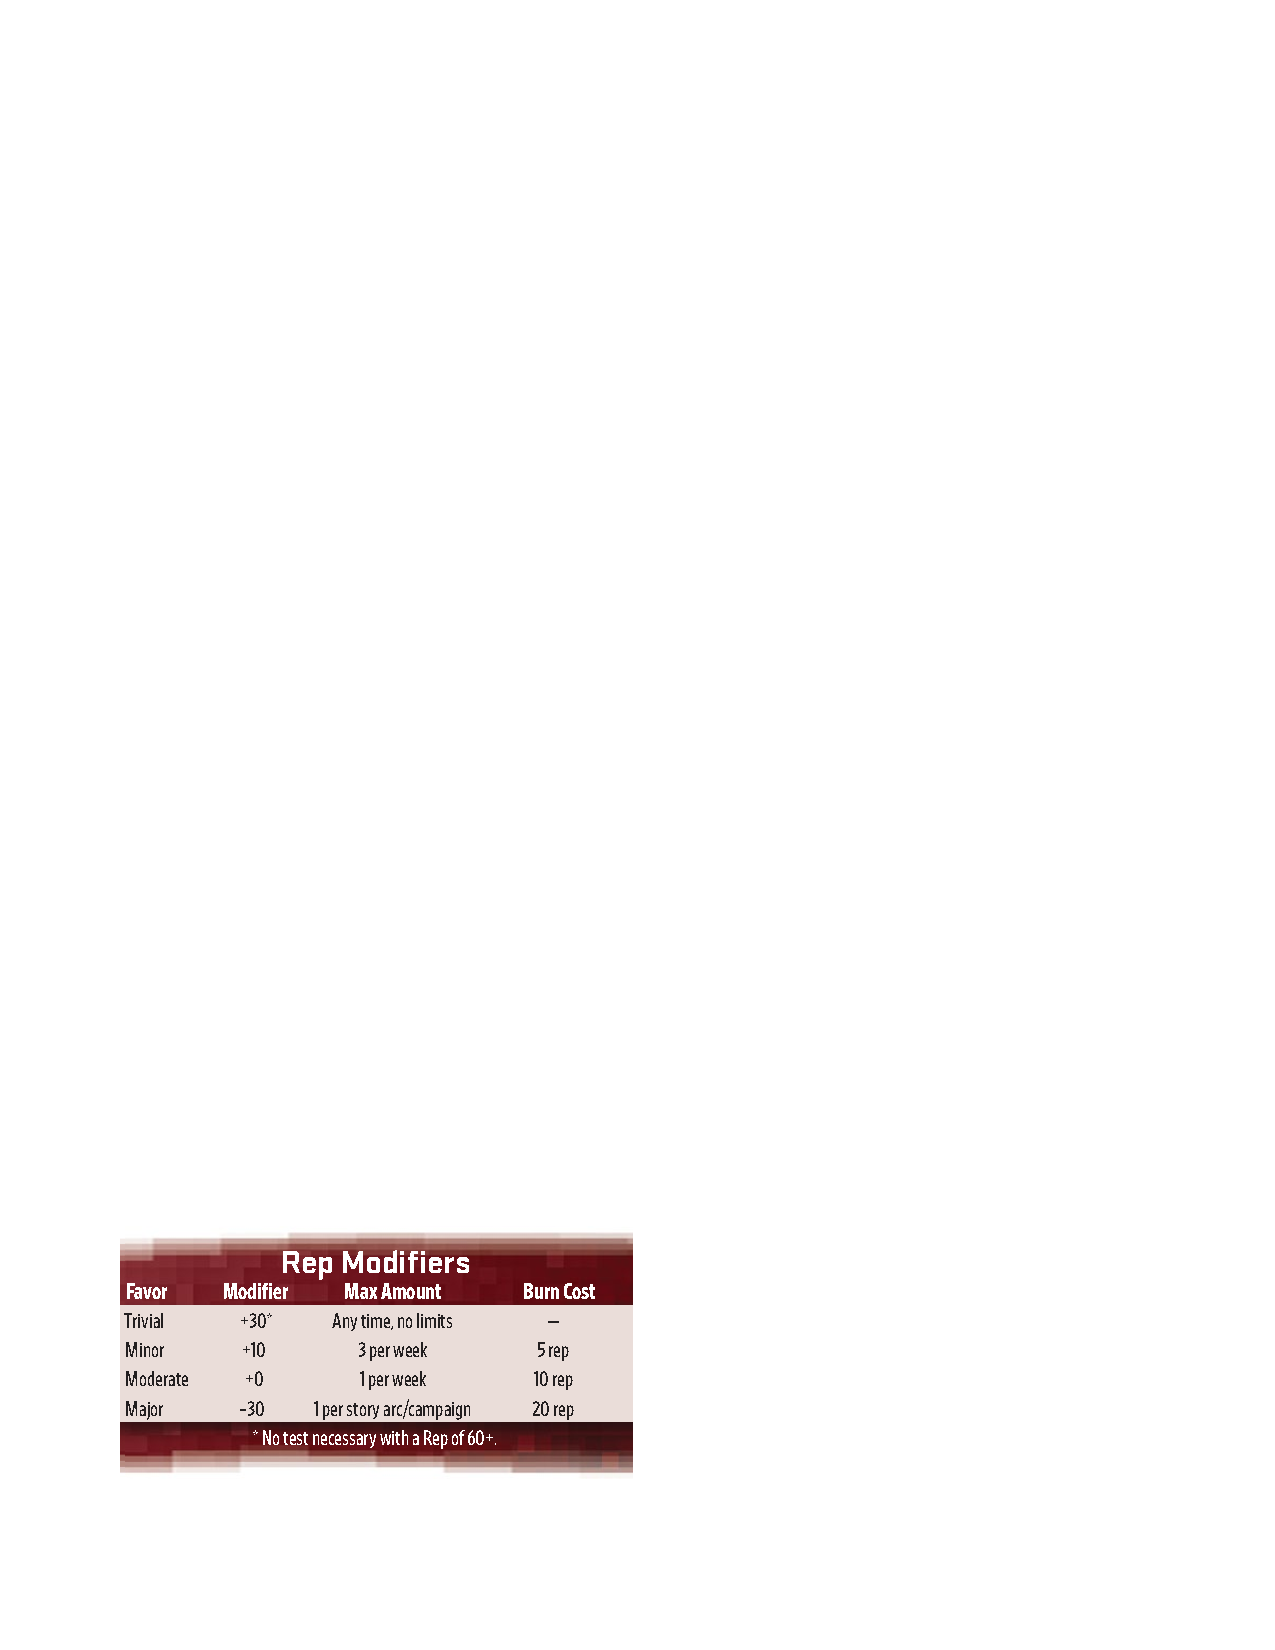
\includegraphics[scale=1]{gfx/resources-rep-cost}%
\end{figure}%

\begin{itemize}
    \itembox \textbf{Rolling Rep}. Look up favor type, apply modifiers and make test in appropriate network. Favor is not lost on failed test unless critical failure is rolled.
    \itembox \textbf{Burning Rep}. Can burn rep to either get favor spent, or get bonus on roll equal to $2x$ the rep burned.
    \itembox \textbf{Keeping Quiet}. For each -X on roll, opponent gets -X to trace.
\end{itemize}
